\section{Durchführung}
\label{sec:Durchführung}
Für die Bestimmung der Zeitabhängigkeit der Amplitude und des effektiven Dämpfungswiderstandes wird der folgende Aufbau der Schaltung in Abbildung \ref{fig:zeit} analysiert.
\begin{figure}[h!]
	\centering
	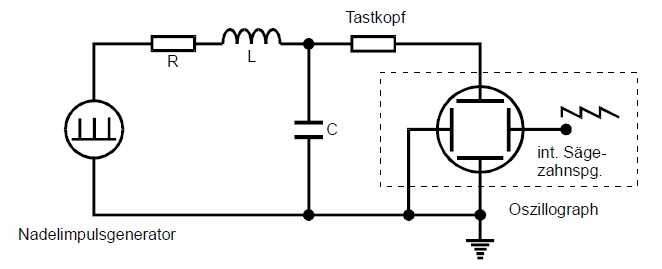
\includegraphics[width=0.7\linewidth]{Zeit.jpg}
	\caption{Aufbau der Schaltung für die Bestimmung der Zeitabhängigkeit der Amplitude sowie des effektiven Dämpfungswiderstandes, \cite[11]{anleitung354}.}
	\label{fig:zeit}
\end{figure}
Zur Messung wird zuerst der Nadelimpulsgenerator so gewählt, dass die Spannungsamplitude etwa um den Faktor $3$ bis $8$ abgesunken ist. Danach wird den Verlauf der Schwingungskurve gegen die Zeit abgetragen. 
Für jede Spannungsamplitude wird die Cursor-Funktion des Oszilloskopes benötigt. Es werden $15$ Werte für die Spannungsamplituden und die Zeit $t$ aufgeschrieben. Zuletzt wird vom angezeigten Bild ein Thermodruck angefertigt.

Zur Messung des Dämpfungswiderstandes $R_{\text{ap}}$, bei dem aperiodischen Grenzfall eintritt, wird die Schaltung aus der Abbildung \ref{fig:widerstand} verwendet.
\begin{figure}[h!]
	\centering
	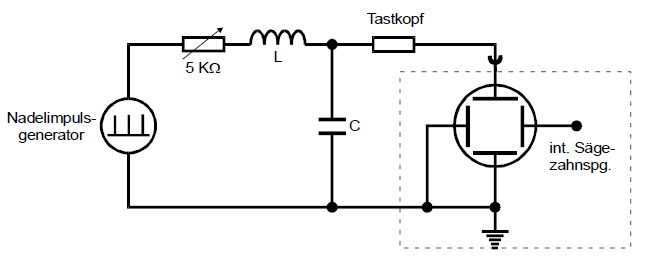
\includegraphics[width=0.7\linewidth]{widerstand.jpg}
	\caption{Aufbau der Schaltung zur Bestimmung des Dämpfungswiderstandes, \cite[12]{anleitung354}.}
	\label{fig:widerstand}
\end{figure}
Der regelbare Widerstand wird auf seinen Maximalwert eingestellt, so dass sich ein Bild für das Relaxationsverhalten eines Schwingkreises ergeben kann. Der Widerstand $R$ wird jetzt solange verringert, bis auf dem
 Bildschirm ein Überschwingen zu sehen ist. Sobald an diesem Punkt das Überschwingen eingetreten ist, muss der Widerstand $R$ wieder erhöht werden, bis das Überschwingen von gerade verschwindet. Als letztes wird der 
 Widerstand $R_{\text{ap}}$ aufgeschrieben.

Zur Bestimmung der Frequenzabhängigkeit der Kondensatorspannung wird eine andere Schaltung gebraucht, die in der Abbildung \ref{fig:frequenz} zu sehen ist. 
\begin{figure}[h!]
	\centering
	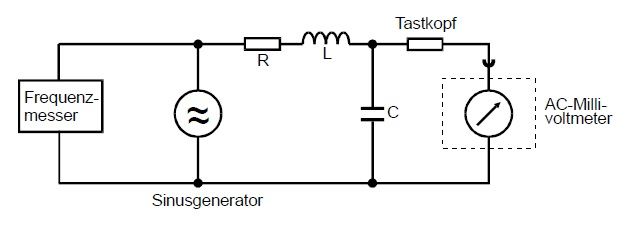
\includegraphics[width=0.7\linewidth]{frequenz.jpg}
	\caption{Aufbau der Schaltung zur Bestimmung der Frequenzabhängigkeit der Kondensatorspannung, \cite[12]{anleitung354}.}
	\label{fig:frequenz}
\end{figure}
Am Sinusgenerator werden Frequenzen im Bereich von $(15-60)\si{\kHz}$ gewählt und es werden 10 Wertepaare für Spannung und Frequenz aufgeschrieben. In diesem Bereich tritt außerdem die Resonanz auf, 
die genauer betrachtet werden soll. Dabei wird diese in $\SI{1}{\kHz}$-Schritten im Bereich von $(30-40)\si{\kHz}$ gemessen und dabei die entsprechende Werte wieder notiert.
Am Ende wird auch die Generatorspannung in Abhängigkeit von Frequenz gemessen und notiert.

Zur Messung der frequenzabhängigen Phasenverschiebung wird die Schaltung wie in Abbildung \ref{fig:freqab} aufgebaut. 
\begin{figure}[h!]
	\centering
	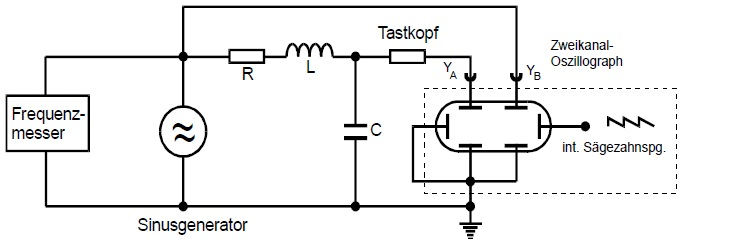
\includegraphics[width=0.7\linewidth]{freqab.jpg}
	\caption{Aufbau der Schaltung zur Bestimmung der Phasenverschiebung bei einem RCL-Kreis, \cite[13]{anleitung354}.}
	\label{fig:freqab}
\end{figure}
Am Oszilloskop ist nun die Generator- und die Kondensatorspannung in Abhängigkeit von Frequenz zu sehen. Wie in der vorherigen Messung werden nacheinander die Frequenzen im Intervall 
von $(15-60)\si{\kHz}$ eingestellt und die Phasenverschiebung der beiden Kurven bestimmt, indem mit dem Cursor der Abstand a gemessen wird. Da in diesem Fall wieder die Resonanzfrequenz eintreten kann, wird diese 
in $\SI{1}{\kHz}$-Schritten im Bereich von $(30-40)\si{\kHz}$ gemessen und dabei die entsprechende Werte wieder notiert. Es ergibt sich ein Bild wie in Abbildung \ref{fig:abstaende}. Der Abstand b kann aus der Frequenz
bestimmt werden.
\begin{figure}[h!]
	\centering
	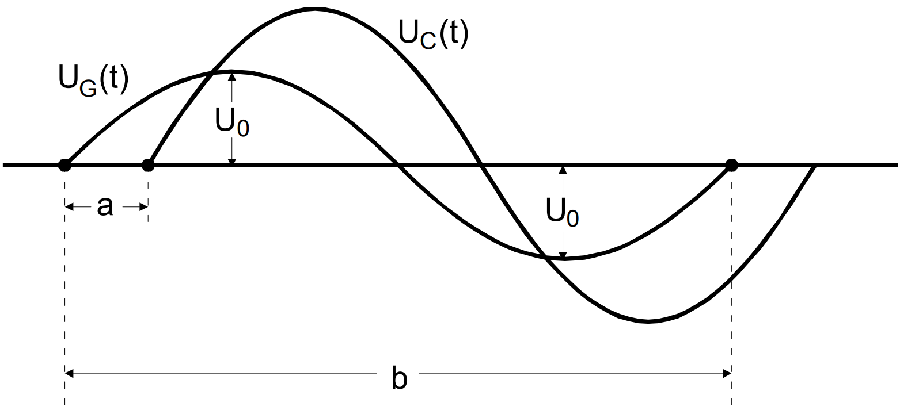
\includegraphics[width=0.7\linewidth]{Abstaende.png}
	\caption{Darstellung des Ozilloskopes der beiden Kurven, \cite[7]{anleitung353}.}
	\label{fig:abstaende}
\end{figure}

